\documentclass[11pt, a4paper, oneside]{book}
\usepackage[margin=2.5cm]{geometry}

\usepackage[portuguese]{babel}

\usepackage[utf8]{inputenc}
\usepackage[x11names,table]{xcolor}
\usepackage{graphicx}
\usepackage[toc,page]{appendix}

\usepackage[binary-units=true]{siunitx}
\sisetup{
    range-phrase=--,
    range-units=single,
    group-separator = {\,}
}
\DeclareSIUnit{\euro}{\mbox{€}}
\usepackage{svg}
\usepackage[hyphens]{url}
\usepackage{hyperref}
\usepackage{caption}
\usepackage{subcaption}
\usepackage{glossaries}
\usepackage{titlepic}
\usepackage{lmodern}
\renewcommand{\familydefault}{\sfdefault}
\usepackage{pdfpages}
\usepackage{fancyhdr}
\usepackage{tikz}
\usepackage{titlesec}
\usepackage{enumitem}
\usepackage{mdframed}
\usepackage{lipsum}

\usepackage{pifont}
\newcommand*\checkmark{%
  \ding{52}%
}

\setlength{\parskip}{0.20\baselineskip}%

\newcommand{\email}[1]{\texttt{#1}}

\pagestyle{fancy}
\fancyhf{}
\renewcommand{\headrulewidth}{0pt}
\fancyhead[R]{
\includegraphics[width=2.0em]{img/recycle-it.png}}
\fancyfoot[C]{\thepage}
\setlength{\headheight}{28pt}
\setlength{\headsep}{10pt}

\definecolor{ourdarkgreen}{HTML}{216942}
\definecolor{ourgreen}{RGB}{44, 142, 90}
\definecolor{ourlightgreen}{HTML}{4AB27B}
\definecolor{ourlightestgreen}{HTML}{7FBF9D}
\definecolor{strengthgreen}{HTML}{00e804}

\titleformat
{name=\chapter,numberless} % command
[block] % shape
{
    \begin{tikzpicture}[remember picture,overlay]
        \fill[ourgreen](-25mm,22mm) rectangle ++(218mm, -30mm);
    \end{tikzpicture}
    \bfseries\Large
} % format
{
} % label
{0.5ex} % sep
{
    \fontsize{30}{30}\selectfont
    \hspace{-10.3mm}
    \color{white}
} % before-code
[
] % after-code
\titlespacing*{name=\chapter,numberless}{0pt}{-1mm}{20mm}

\titleformat
{\chapter} % command
[block] % shape
{
    \begin{tikzpicture}[remember picture,overlay]
        \fill[ourgreen](-25mm,35.5mm) rectangle ++(218mm, -50mm);
        \fill[white](-25mm,27.5mm) rectangle ++(34mm, -34mm);
        \draw(-3mm,8.5mm) node[color=ourgreen, align=left] {\bfseries \fontsize{70}{70}\selectfont \thechapter};
    \end{tikzpicture}
    \bfseries\Large
} % format
{
} % label
{0.5ex} % sep
{
    \fontsize{30}{30}\selectfont
    \hspace{8mm}
    \color{white}
} % before-code
[
] % after-code
\titlespacing*{\chapter}{0pt}{14mm}{25mm}

\makeatletter
\def\printauthor{{\@author}}
\makeatother

\makeatletter
\def\printtitle{{\@title}}
\makeatother

\makeatletter
\def\printdate{{\@date}}
\makeatother

\makeatletter
\def\printinstitution{%
Mestrado Integrado em Engenharia Informática e Computação \\
3º ano, 2º semestre \\
Proficiência Pessoal e Interpessoal
}
\makeatother

% Copyright page
\newenvironment{secondpage}{
    \clearpage\null\vfill
    \thispagestyle{empty}
    \begin{minipage}[b]{0.9\textwidth}
        \footnotesize\raggedright
        \setlength{\parskip}{0.5\baselineskip}
}{
    \end{minipage}
    \vspace*{2\baselineskip}
}

% Metadata
\title{
\includegraphics[scale=0.2]{img/recycle-it-full-white.png}}
\author{
    \hspace{-3.4mm}
    \begin{tabular}{@{} l l @{}}
        Diogo Miguel Ferreira Rodrigues & (\email{up201806429@edu.fe.up.pt}) \\
        Iohan Xavier Sardinha Dutra Soares & (\email{up201801011@edu.fe.up.pt}) \\
        João António Cardoso Vieira e Basto de Sousa & (\email{up201806613@edu.fe.up.pt}) \\
        Pedro Daniel Fernandes Ferreira & (\email{up201806506@edu.fe.up.pt}) \\
        Pedro Varandas da Costa Azevedo da Ponte & (\email{up201809694@edu.fe.up.pt})
    \end{tabular}
}
\date{6 de Junho de 2021}

\makeglossaries
\newglossaryentry{rsu}{
    name=resíduo sólido urbano,
    description={Designado abreviadamente de RSU, é um objeto ou substância sólida que, na sua condição atual, não possui utilidade para quem o detém, pelo que deve ser descartado de forma adequada. Não possuir utilidade para quem o detém não significa que não tenha valor económico: não só as matérias-primas do qual o RSU é feito possuem geralmente valor económico, como o RSU pode ser útil a outra pessoa ou empresa que seja capaz de reutilizar/reciclar o RSU. Neste documento os termos "lixo" e "resíduos" são usados como sinónimos de RSU}
}
\newglossaryentry{lixo}{
    name=lixo,
    description={Equivalente a resíduo sólido urbano}
}
\newglossaryentry{entidade gestora}{
    name=entidade gestora,
    description={Entidade que gere a recolha e tratamento dos resíduos sólidos urbanos numa determinada zona; pode-se tratar, por exemplo, de um município, de uma empresa municipal especializada, ou de uma entidade trans-municipal \cite{dl-152d-2017}}
}
\newglossaryentry{justica ambiental}{
    name=justiça ambiental,
    description={Termo utilizado para enquadrar os problemas ambientais (aquecimento global, poluição, destruição de habitat) como questões éticas e políticas, e não apenas como questões ambientais ou físicas. Geralmente refere-se à forma injusta como diferentes países e classes sociais são afetados por problemas ambientais originados pela forma como a sociedade de consumo mundial opera, pelo que a justiça ambiental é atingida quando cada pessoa é responsabilizada, tributada ou processada judicialmente em proporção com o impacto negativo que tem no meio ambiente}
}

\usepackage[utf8]{inputenc}
\usepackage{array, booktabs}
\usepackage{graphicx}

\newcommand{\foo}{\color{ourgreen}\makebox[0pt]{\Large$\bullet$}\hskip-1pt\vrule width 2pt\hspace{\labelsep}}

\linespread{1.075}
\begin{document}

\begin{titlepage}
    \begin{tikzpicture}[remember picture,overlay]
        \begin{scope}[shift={(-31mm, 10mm)}]
            \draw[fill=ourgreen, ourgreen]
                  (0, 0) rectangle ++(210mm, -52mm);
        \end{scope}
    \end{tikzpicture}
    \begin{tikzpicture}[remember picture,overlay]
        \begin{scope}[shift={(177.7mm, 10mm)}, scale=2]
            \draw[fill=ourdarkgreen, ourdarkgreen]
                  (0, 0) rectangle ++(-1, -1);
            \draw[fill=ourlightestgreen, ourlightestgreen]
                  (-1, +0) node[]{} --
                ++(-1, +0) node[]{} --
                ++(+0, -1) node[]{} -- cycle;
            \draw[fill=ourlightgreen, ourlightgreen]
                  (-1, +0) node[]{} --
                ++(+0, -1) node[]{} --
                ++(-1, +0) node[]{} -- cycle;
            \draw[fill=ourdarkgreen, ourdarkgreen]
                  (-2, +0) node[]{} --
                ++(+0, -1) node[]{} --
                ++(-1, +1) node[]{} -- cycle;
            \draw[fill=ourlightestgreen, ourlightestgreen]
                  (-1, -1) node[]{} --
                ++(+1, +0) node[]{} --
                ++(+0, -1) node[]{} -- cycle;
        \end{scope}
    \end{tikzpicture}
    \begin{tikzpicture}[remember picture,overlay]
        \draw(-15mm,-15mm) node[anchor=west] {\printtitle};
    \end{tikzpicture}
    \begin{tikzpicture}[remember picture,overlay]
        \draw(-15mm,-70mm) node[anchor=west] {\bfseries \Huge Relatório do projeto};
    \end{tikzpicture}
    \begin{tikzpicture}[remember picture,overlay]
        \draw(-15mm,-97mm) node[anchor=west, align=left] {
            \printauthor
        };
    \end{tikzpicture}
    \begin{tikzpicture}[remember picture,overlay]
        \draw(-17mm,-115mm) node[anchor=north west, align=left] {
            \printinstitution
        };
    \end{tikzpicture}
    \begin{tikzpicture}[remember picture,overlay]
        \draw(+70mm,-250mm) node[anchor=south, align=center] {
            % \includesvg[scale=0.3]{img/minerva.svg} \\
            
\includegraphics[scale=0.4]{img/feup.png} \\[2em]
        
            % Faculdade de Engenharia da Universidade do Porto \\
            Porto, Portugal \\
            \printdate
        };
    \end{tikzpicture}
\end{titlepage}
\pagecolor{white}
        
\begin{secondpage}
    Copyright \copyright 2021--\the\year\ Diogo Rodrigues, João António Sousa, Pedro Ferreira, Pedro Ponte, Iohan Soares\par
    É permitida a cópia e redistribuição deste documento sob os termos da licença pública
    \href{https://creativecommons.org/licenses/by-nc-nd/4.0/}{Creative Commons Attribution-NonCommercial-NoDerivatives 4.0 International}.\par
    
    \vspace{2em}
    
    Autores: \par
    \begin{tabular}{@{} l l @{}}
        Diogo Miguel Ferreira Rodrigues & (\email{up201806429@edu.fe.up.pt}) \\
        Iohan Xavier Sardinha Dutra Soares & (\email{up201801011@edu.fe.up.pt}) \\
        João António Cardoso Vieira e Basto de Sousa & (\email{up201806613@edu.fe.up.pt}) \\
        Pedro Daniel Fernandes Ferreira & (\email{up201806506@edu.fe.up.pt}) \\
        Pedro Varandas da Costa Azevedo da Ponte & (\email{up201809694@edu.fe.up.pt})
    \end{tabular}\par
    
    \vspace{2em}

    Realizado sob supervisão da Professora Fernanda Maria dos Santos Teixeira Torres.
\end{secondpage}

\frontmatter

{
\linespread{1.000}

\tableofcontents
}

\mainmatter

\nocite{*}
\bibliographystyle{acm}
\clearpage
\addcontentsline{toc}{chapter}{Bibliografia}
\bibliography{references}

% https://www.lipor.pt/darmais/faq/gestao-residuos.html

% https://apambiente.pt/index.php?ref=16&subref=84&sub2ref=933&sub3ref=936

\renewcommand{\appendixtocname}{Anexos}
\renewcommand{\appendixpagename}{Anexos}
\begin{appendices}
\chapter{Ficha técnica}

Este projeto foi proposto no contexto da unidade curricular de Proficiência Pessoal e Interpessoal (PPIN), no segundo semestre do terceiro ano curricular do curso de Mestrado Integrado em Engenharia Informática e Computação (MIEIC) da Faculdade de Engenharia da Universidade do Porto (FEUP), com o objetivo de cumprimento parcial do elemento de avaliação "Projeto de Inovação", sob orientação da Professora Fernanda Torres.

\section{Elementos do grupo}

Todos os elementos do grupo pertencem à turma 7.

\begin{center}
\begin{tabular}{@{} l l@{}}
    \textbf{Elemento do grupo} & \textbf{Número mecanográfico} \\ \hline
    Diogo Miguel Ferreira Rodrigues & 201806429 \\
    Iohan Xavier Sardinha Dutra Soares & 201806429 \\
    João António Cardoso Vieira e Basto de Sousa & 201806613 \\
    Pedro Daniel Fernandes Ferreira & 201806506 \\
    Pedro Varandas da Costa Azevedo da Ponte & 201809694
\end{tabular}
\end{center}

\section{Funcionamento do grupo e dos seus elementos}

Julgamos que o grupo responsável por desenvolver este projeto teve boa interação e que todos os membros estiveram ao nível das elevadas expectativas que foram definidas pelo grupo. Todos os membros tiveram contribuições importantes e decisivas para este projeto, e o esforço colocado neste projeto foi semelhante entre alunos, mesmo que esse esforço não seja possível colocar inteiramente por escrito na secção seguinte.

Desta forma, entendemos que, em jeito de heteroavaliação, não há nada a apontar a nenhum membro do grupo em particular. Em termos de autoavaliação, o trabalho desenvolvido é entendido como completo e relevante, apesar de ter sido realizado sob circunstâncias tão difíceis como a dificuldade inerente ao semestre em que a unidade curricular de PPIN se enquadra (que deriva da dificuldade global de todas as unidades curriculares desse semestre), além da situação provocada pela pandemia COVID-19 que dificulta alguns contactos mais informais que seriam comuns em horas de aula e intervalos; este desafio foi parcialmente ultrapassado através da utilização da ferramenta Discord para envio de mensagens instantâneas e chamadas de voz.

\newpage

\section{Descrição das tarefas realizadas}

\begin{center}
    \begin{tabular}{@{} p{12.9em}|p{4.6em}|p{4.6em}|p{4.6em}|p{4.6em}|p{4.6em} @{}}
        & \textbf{Diogo ~ Rodrigues} & \textbf{Iohan ~ Soares} & \textbf{João António Sousa} & \textbf{Pedro Ferreira} & \textbf{Pedro Ponte} \\ \hline
        \textbf{Apresentação intermédia} & & & & \\
        Design dos diapositivos & \checkmark & & & & \\
        Apresentação & & & \checkmark & & \\ \hline
        \textbf{Apresentação final} & & & & \\
        Design dos diapositivos & \checkmark & & & \checkmark & \\
        Introdução & & & & \checkmark & \\
        Informações recolhidas & & & & \checkmark & \\
        Metas e oportunidades & & \checkmark & \checkmark & & \\
        Soluções tecnológicas & \checkmark & & & & \\
        Descrição do projeto & & & & \\
        ~~ Funcionamento & \checkmark & & & & \checkmark \\
        ~~ Aplicação & & & \checkmark & & \\
        Análise da concorrência & \checkmark & & & & \\
        Modelo de negócio & & & \checkmark & & \\
        Plano de ação & & & & & \checkmark \\ \hline
        \textbf{Relatório} & & & & & \\
        Design do relatório & \checkmark & & & & \\
        Introdução & \checkmark & \checkmark & \checkmark & \checkmark & \checkmark \\
        Revisão bibliográfica & & & & & \\
        ~~ Evidência e legislação & & \checkmark & \checkmark & & \\
        ~~ Soluções tecnológicas & \checkmark & & & & \\
        Descrição do projeto & & & & & \\
        ~~ Sistema centralizado & \checkmark & & & & \\
        ~~ Recolha de resíduos & \checkmark & & & & \checkmark \\
        ~~ Aplicação móvel & \checkmark & & \checkmark & & \\
        ~~ Modo de operação & \checkmark & & & & \\
        ~~ Estudo da concorrência & \checkmark & & & & \\
        ~~ Análise SWOT & \checkmark & & & & \\
        Modelo de negócio & & & \checkmark & \\
        Plano de ação & & & & & \checkmark \\
        Conclusão & \checkmark & \checkmark & \checkmark & \checkmark & \checkmark \\
        Anexos & & & & & \\
        ~~ Resultados do questionário & & & & \checkmark & \\
        ~~ Diário de bordo & & \checkmark & & \\ \hline
        \textbf{Outros} & & & & & \\
        Logótipo & & & \checkmark & & \\
        Questionário & & & & \checkmark & \\
    \end{tabular}
\end{center}

% ficha técnica - elementos do grupo, descrição dos papéis e tarefas realizadas por cada um, bem como uma análise crítica do grupo sobre a forma como decorreu o trabalho da equipa (auto e hétero-avaliação)

\chapter{Questionário e resultados}

Foi efetuado um questionário para melhor conhecer a opinião das pessoas em relação aos problemas que o nosso projeto pretende resolver e à solução apresentada, assim como disponibilizar um espaço de sugestões.

\section{Questionário}

\subsection{Secção 1}

\begin{mdframed}[innerleftmargin=7.5mm, innerrightmargin=7.5mm, innertopmargin=7.5mm, innerbottommargin=7.5mm]

\setlength{\parindent}{0pt}

{\Large \textbf{Inquérito PPIN - RecycleIt}}

~

16 de maio de 2021 \\
Faculdade de Engenharia da Universidade do Porto

~

Hoje em dia, há uma crescente preocupação com a separação dos resíduos. Contudo, os incentivos para este comportamento não são atrativos. De forma geral, a única recompensa garantida é o reconhecimento próprio de se estar a não contribuir para um aumento do desperdício e consequente poluição do ambiente. As taxas de resíduos sólidos não têm em conta esta situação, não havendo nenhum impacto direto no ato de separar corretamente.

~

A RecycleIt tem em vista o aumento da separação correta dos resíduos por parte dos cidadãos em prol da justiça ambiental que promove um grau de reciclagem de resíduos mais elevado, recompensando os "participantes" com parte das receitas que a entidade gestora de resíduos obtém com esta mudança de comportamentos, ou seja, originaria não só benefícios para o ambiente como também para as pessoas que reciclam.

~

Para tal, gostaríamos da sua colaboração neste inquérito de 1 minuto, de modo a aferir quais as mais-valias do serviço apresentado e melhorar a qualidade e rentabilidade deste.

~

Obrigado pela sua colaboração!
\end{mdframed}

\newpage

\subsection{Secção 2}

\setlength{\parindent}{0pt}

\begin{mdframed}[innerleftmargin=7.5mm, innerrightmargin=7.5mm, innertopmargin=7.5mm, innerbottommargin=7.5mm]

{\Large \textbf{Inquérito PPIN - RecycleIt}}

~

Faz separação e reciclagem de lixo?
\begin{itemize}[label={\huge $\circ$}]
    \itemsep0em
    \item Sim
    \item Não
    \item Às vezes
\end{itemize}
\vspace{-0.7em}\rule{\linewidth}{0.5pt}\vspace{0.5em}

Como é que variaram os seus hábitos de reciclagem de lixo desde o início da pandemia?
\begin{center}
    \begin{tabular}{l c c c r}
         & 1 & 2 & 3 & \\[0.5em]
         Diminuíram & {\huge$\circ$} & {\huge$\circ$} & {\huge$\circ$} & Aumentaram
    \end{tabular}
\end{center}
\vspace{-0.1em}\rule{\linewidth}{0.5pt}\vspace{0.5em}

Qual considera a maior razão para a não reciclagem de lixo?
\begin{itemize}[label={\huge $\circ$}]
    \itemsep0em
    \item Falta de ecopontos
    \item Falta de hábito
    \item Não haver incentivos
    \item Dá muito trabalho
\end{itemize}
\vspace{-0.7em}\rule{\linewidth}{0.5pt}\vspace{0.5em}

Qual a sua opinião em relação aos atuais incentivos à reciclagem?
\begin{center}
    \begin{tabular}{l c c c c c r}
         & 1 & 2 & 3 & 4 & 5 & \\[0.5em]
         Inexistentes & {\huge$\circ$} & {\huge$\circ$} & {\huge$\circ$} & {\huge$\circ$} & {\huge$\circ$} & Muito bons
    \end{tabular}
\end{center}
\vspace{-0.1em}\rule{\linewidth}{0.5pt}\vspace{0.5em}

Qual a sua opinião em relação ao valor das taxas de resíduos sólidos?
\begin{center}
    \begin{tabular}{l c c c c c r}
         & 1 & 2 & 3 & 4 & 5 & \\[0.5em]
         Muito Insatisfeito & {\huge$\circ$} & {\huge$\circ$} & {\huge$\circ$} & {\huge$\circ$} & {\huge$\circ$} & Muito Satisfeito
    \end{tabular}
\end{center}
\vspace{-0.1em}\rule{\linewidth}{0.5pt}\vspace{0.5em}

Estaria interessado em receber um caixote do lixo de cada tipo de resíduo munido de uma etiqueta e um código QR de identificação da residência, bem como um sistema de abertura dos caixotes que não permitem a utilização dos mesmos por outras pessoas? (Caso habite em apartamentos os caixotes serão de maiores dimensões com um sistema de acesso com cartão para abrir o contentor e uma balança incorporada)
\begin{itemize}[label={\huge $\circ$}]
    \itemsep0em
    \item Sim
    \item Não
\end{itemize}
\vspace{-0.7em}\rule{\linewidth}{0.5pt}\vspace{0.5em}

Estaria interessado numa app que permitisse aos utilizadores serem avisados com antecedência sobre quando serão as próximas recolhas de lixo?
\begin{itemize}[label={\huge $\circ$}]
    \itemsep0em
    \item Sim
    \item Não
\end{itemize}
\vspace{-0.7em}\rule{\linewidth}{0.5pt}\vspace{0.5em}

Estaria interessado numa app que permitisse consultar a quantidade de resíduos produzidos e o seu processo de recolha para pagar um valor proporcional aos resíduos produzidos?
\begin{itemize}[label={\huge $\circ$}]
    \itemsep0em
    \item Sim
    \item Não
\end{itemize}
\vspace{-0.7em}\rule{\linewidth}{0.5pt}\vspace{0.5em}

Estaria interessado numa campanha que permitisse ser recompensado com parte das receitas que a entidade gestora de resíduos obtém por reciclar corretamente os seus resíduos?
\begin{itemize}[label={\huge $\circ$}]
    \itemsep0em
    \item Sim
    \item Não
\end{itemize}
\vspace{-0.7em}\rule{\linewidth}{0.5pt}\vspace{0.5em}

Tem alguma sugestão que poderia acrescentar algo que considera relevante ao projeto de inovação?

~

\noindent\fbox{\parbox{\linewidth - 7pt}{%
    ~
    
    ~
    
    ~
}}

\end{mdframed}

\newpage

\section{Processo de recolha de resultados}

O questionário foi realizado através de Google Forms. Todas as perguntas são obrigatórias exceto a última pergunta, que apenas deve ser respondida de forma opcional com sugestões.

O link do questionário foi enviado a 9044 alunos da Faculdade de Engenharia da Universidade do Porto, no dia 16 de Maio de 2021 às 13:18. Até ao dia 19 de Maio de 2021 às 23:59, havia 159 respostas, e até ao dia 5 de Junho às 20:00 o questionário foi respondido 162 vezes, momento a partir do qual considerámos a fase de recolha de resultados terminada.

\section{Resultados completos}

\begin{mdframed}[innerleftmargin=7.5mm, innerrightmargin=7.5mm, innertopmargin=7.5mm, innerbottommargin=7.5mm]

{\Large \textbf{Inquérito PPIN - RecycleIt}}

~

Faz separação e reciclagem de lixo?

~

\begin{tabular}{@{} l | r r @{} }
    \textbf{Opção} & \textbf{Resultados} & \textbf{(\%)} \\ \hline
    Sim      & 126 & (77.8\%) \\
    Não      &  10 & ( 6.2\%) \\
    Às vezes &  26 & (16.0\%) 
\end{tabular}

~

\rule{\linewidth}{0.5pt}\vspace{0.5em}

Como é que variaram os seus hábitos de reciclagem de lixo desde o início da pandemia?

~

\begin{tabular}{@{} l | r r @{} }
    \textbf{Opção} & \textbf{Resultados} & \textbf{(\%)} \\ \hline
    1 (diminuíram) &   6 & ( 3.7\%) \\
    2              & 122 & (75.3\%) \\
    3 (aumentaram) &  34 & (21.0\%)
\end{tabular}

~

\rule{\linewidth}{0.5pt}\vspace{0.5em}

Qual considera a maior razão para a não reciclagem de lixo?

~

\begin{tabular}{@{} l | r r @{} }
    \textbf{Opção} & \textbf{Resultados} & \textbf{(\%)} \\ \hline
    Falta de ecopontos   &  19 & (11.7\%) \\
    Falta de hábito      &  94 & (58.0\%) \\
    Não haver incentivos &  32 & (22.2\%)  \\
    Dá muito trabalho    &  13 & ( 8.0\%)
\end{tabular}

~

\rule{\linewidth}{0.5pt}\vspace{0.5em}

Qual a sua opinião em relação aos atuais incentivos à reciclagem?

~

\begin{tabular}{@{} l | r r @{} }
    \textbf{Opção} & \textbf{Resultados} & \textbf{(\%)} \\ \hline
    1 (inexistentes) &  35 & (21.6\%) \\
    2                &  59 & (36.4\%) \\
    3                &  51 & (31.5\%) \\
    4                &  15 & ( 9.3\%) \\
    5 (muito bons)   &   2 & ( 1.2\%)
\end{tabular}

~

\rule{\linewidth}{0.5pt}\vspace{0.5em}

Qual a sua opinião em relação ao valor das taxas de resíduos sólidos?

~

\begin{tabular}{@{} l | r r @{} }
    \textbf{Opção} & \textbf{Resultados} & \textbf{(\%)} \\ \hline
    1 (muito insatisfeito) &  18 & (11.1\%) \\
    2                      &  40 & (24.7\%) \\
    3                      &  96 & (59.3\%) \\
    4                      &   7 & ( 4.3\%) \\
    5 (muito satisfeito)   &   1 & ( 0.6\%)
\end{tabular}

~

\rule{\linewidth}{0.5pt}\vspace{0.5em}

Estaria interessado em receber um caixote do lixo de cada tipo de resíduo munido de uma etiqueta e um código QR de identificação da residência, bem como um sistema de abertura dos caixotes que não permitem a utilização dos mesmos por outras pessoas? (Caso habite em apartamentos os caixotes serão de maiores dimensões com um sistema de acesso com cartão para abrir o contentor e uma balança incorporada)

~

\begin{tabular}{@{} l | r r @{} }
    \textbf{Opção} & \textbf{Resultados} & \textbf{(\%)} \\ \hline
    Sim & 130 & (80.2\%) \\
    Não &  32 & (19.8\%) \\
\end{tabular}

~

\rule{\linewidth}{0.5pt}\vspace{0.5em}

Estaria interessado numa app que permitisse aos utilizadores serem avisados com antecedência sobre quando serão as próximas recolhas de lixo?

~

\begin{tabular}{@{} l | r r @{} }
    \textbf{Opção} & \textbf{Resultados} & \textbf{(\%)} \\ \hline
    Sim & 131 & (80.9\%) \\
    Não &  31 & (19.1\%) \\
\end{tabular}

~

\rule{\linewidth}{0.5pt}\vspace{0.5em}

Estaria interessado numa app que permitisse consultar a quantidade de resíduos produzidos e o seu processo de recolha para pagar um valor proporcional aos resíduos produzidos?

~

\begin{tabular}{@{} l | r r @{} }
    \textbf{Opção} & \textbf{Resultados} & \textbf{(\%)} \\ \hline
    Sim & 136 & (84.0\%) \\
    Não &  26 & (16.0\%) \\
\end{tabular}

~

\rule{\linewidth}{0.5pt}\vspace{0.5em}

Estaria interessado numa campanha que permitisse ser recompensado com parte das receitas que a entidade gestora de resíduos obtém por reciclar corretamente os seus resíduos?

~

\begin{tabular}{@{} l | r r @{} }
    \textbf{Opção} & \textbf{Resultados} & \textbf{(\%)} \\ \hline
    Sim & 153 & (94.4\%) \\
    Não &   9 & ( 5.6\%) \\
\end{tabular}

~

\rule{\linewidth}{0.5pt}\vspace{0.5em}

Tem alguma sugestão que poderia acrescentar algo que considera relevante ao projeto de inovação?

~

{\color{black!75}Nota: Esta pergunta foi respondida 18 vezes. Foram removidas todas as respostas sim/não (1), fora de contexto (1) ou com linguagem insultuosa (1), resultando em 15 respostas válidas. Relativamente às respostas válidas, foram apenas corrigidos erros gramaticais.}

~

\noindent\fbox{\parbox{\linewidth - 7pt}{%
Gostava de poder comprar stocks, ações de empresas de gestão e reciclagem de resíduos. Se contribuo para a sua produção, porque não ganhar com o seu crescimento?
}}

\noindent\fbox{\parbox{\linewidth - 7pt}{%
Parcerias com instituições de caridade ou empresas que aproveitassem os resíduos para intuitos caridosos (ex: tampinhas das garrafas recolhidas para conversão em cadeiras de rodas).
}}

\noindent\fbox{\parbox{\linewidth - 7pt}{%
Às vezes é complicado saber quais produtos devem ser colocados em determinado ecoponto. A app podia ter uma secção que nos dissesse quais produtos iam para qual ecoponto, de uma forma mais particular, por exemplo os pacotes de leite.
}}

\noindent\fbox{\parbox{\linewidth - 7pt}{%
Motivação e falta de sentir progresso/propósito em reciclar são os maiores impasses na reciclagem, a meu ver. Assim sendo, iniciativas ou medidas que incentivem a reciclagem e que tragam um benefício a quem recicla são muito importantes.
}}

\noindent\fbox{\parbox{\linewidth - 7pt}{%
Olhar p/ resíduos como um bem com valor reciclável (pelo qual pagou ao comprar o produto) em vez de um custo.
}}

\noindent\fbox{\parbox{\linewidth - 7pt}{%
Opção de doar os "ganhos" para uma iniciativa de caridade à escolha do utilizador.
Existe em Portugal um projeto de caridade que consiste em trocar tampas de plástico por cadeiras de rodas para quem mais necessita, que ao longo dos anos contribuiu bastante para o aumento da reciclagem por parte dos portugueses. Sinceramente, penso que os ganhos que se obteria como recompensa pela reciclagem por parte de entidades gestoras de resíduos não seriam quase nada. Seriam uns trocos. Não sei até que ponto valeria a pena. Mas se adicionarem a opção de ajudar uma iniciativa de caridade, o conjunto dos trocos que se juntam de cada recompensa individual poderia contribuir significativamente para uma causa de caridade. No caso das tampas de plástico, numa casa vão se juntando umas 20-30 tampinhas por mês, mas quando várias pessoas se juntam, já se chega às toneladas, que permitem doar dezenas de cadeiras de rodas a quem precisa. Se usarem o exemplo das tampinhas como \textit{proof of concept}, penso que conseguem dar poder ao vosso projeto e convencer os vossos colegas e professores que a vossa app poderá contribuir para o aumento da reciclagem. (E com a caridade teriam mais uma dimensão que aumentaria o valor moral da vossa app).
}}

\noindent\fbox{\parbox{\linewidth - 7pt}{%
A maior "motivação"{} para fazer a reciclagem entre outras atividades relacionadas deve ser a consciência e não recompensas monetárias.
}}

\noindent\fbox{\parbox{\linewidth - 7pt}{%
Não que seja o meu caso, mas acho que o português comum tem um mindset de chico-esperto, e que com o controlo da quantidade de lixo produzido iria aumentar a quantidade de pessoas que o descartam de forma imprópria. Vivo perto de uma bouça, e a urbanização estava repleta de encontros para reciclagem, mesmo assim algumas criaturas ainda optavam por ir descartar as suas embalagem no meio dos pinheiros. Se passassem a pagar mais por usar mais os contentores que a câmara lhes distribuiu, ainda recorriam mais a essa prática. É triste, mas se mesmo com tarifa fixa (dependente do consumo de água) preferem deixar o lixo na bouça em vez de por no contentor à porta imaginemos com um sistema onde se paga mais por eliminar no sítio certo/ reciclar maior quantidade de resíduos.
}}

\noindent\fbox{\parbox{\linewidth - 7pt}{%
Multa para quem não separa corretamente o lixo ou coloca fora de tempo (era assim na Bélgica há 15 anos a trás).
}}

\noindent\fbox{\parbox{\linewidth - 7pt}{%
Já existe um projeto parecido na Suíça com a diferença que, em vez de caixotes do lixo com QR codes, as pessoas só podem deitar lixo com sacos específicos que compram ao governo, que funcionam como uma taxa, uma vez que o preço é elevado, para além disto não há sacos de lixo à venda nos supermecados.
}}

\noindent\fbox{\parbox{\linewidth - 7pt}{%
Parece-me algo mais complexo do que poderia ser e para muitos acaba sendo inacessível, é essencial a simplificação ao máximo para abranger todas as faixas etárias e conhecimentos tecnológicos.
}}

\noindent\fbox{\parbox{\linewidth - 7pt}{%
Devolver garrafas e afins nos supermercados em troca de incentivos monetários.
}}

\noindent\fbox{\parbox{\linewidth - 7pt}{%
Percebo a ideia por detrás do método com o código QR, mas creio que pode tornar o processo mais complicado para as pessoas que não são tão adeptas da tecnologia. Pessoalmente, no que toca à reciclagem, quanto mais fácil e conveniente ao utilizador, melhor.
}}

\noindent\fbox{\parbox{\linewidth - 7pt}{%
Direcionar as pessoas para usar menos plástico e mencionar alternativas.
}}

\noindent\fbox{\parbox{\linewidth - 7pt}{%
App permitisse consultar que tipo de resíduo (cartão, plástico, metal..) é o lixo que se quer descartar pois nem sempre é fácil perceber.
}}

\end{mdframed}

\subsection{Reflexões sobre as sugestões}

\noindent\fbox{\parbox{\linewidth}{%
Gostava de poder comprar stocks, ações de empresas de gestão e reciclagem de resíduos. Se contribuo para a sua produção, porque não ganhar com o seu crescimento?
}}

As empresas de gestão de resíduos são geralmente empresas municipais ou trans-municipais, geridas por municípios ou áreas metropolitanas/regiões. Assim, não têm os objetivos comuns das empresas privadas de crescer e distribuir lucros. As empresas de revenda de lixo são geralmente privadas, por isso a possibilidade de transacionar ações dessas empresas depende da sua tipologia, não sendo em particular uma questão que diz respeito a este projeto. De qualquer forma, e como sugerido, as pessoas devem ser recompensadas por separar corretamente o lixo, nomeadamente através da redução de encargos financeiros. No entanto, as pessoas não devem ser recompensadas por produzir mais resíduos, mesmo que corretamente separados, dado que a produção desses resíduos continua a ter um impacto ambiental.

~

\noindent\fbox{\parbox{\linewidth}{%
Parcerias com instituições de caridade ou empresas que aproveitassem os resíduos para intuitos caridosos (ex: tampinhas das garrafas recolhidas para conversão em cadeiras de rodas).
}}

A forma como a entidade gestora distribui os dividendos resultantes da operação de venda do lixo cabe apenas à entidade gestora. No entanto, por exemplo no caso do projeto Recicle Mais, Pague Menos (Maia), as receitas da venda de resíduos separados em 2021 obtidas durante a fase de teste, com 3500 famílias, reverterá para uma instituição de solidariedade \cite{rmpm-noticiasmaia}.

~

\noindent\fbox{\parbox{\linewidth}{%
Às vezes é complicado saber quais produtos devem ser colocados em determinado ecoponto. A app podia ter uma secção que nos dissesse quais produtos iam para qual ecoponto, de uma forma mais particular, por exemplo os pacotes de leite.
}}


\noindent\fbox{\parbox{\linewidth}{%
App permitisse consultar que tipo de resíduo (cartão, plástico, metal..) é o lixo que se quer descartar pois nem sempre é fácil perceber.
}}

Incluímos esta sugestão no nosso projeto.

~

\noindent\fbox{\parbox{\linewidth}{%
A maior "motivação"{} para fazer a reciclagem entre outras atividades relacionadas deve ser a consciência e não recompensas monetárias.
}}

O objetivo deste projeto não é mercantilizar a responsabilidade cívica. O objetivo é tributar as pessoas de acordo com a quantidade que reciclam e a forma como reciclam, um regime vantajoso para quem faz a separação correta dos resíduos e apenas consome na medida do necessário. De qualquer forma, a defesa do ambiente não é uma questão de "consciência", dado que a atividade humana tem um impacto real no meio ambiente; as pessoas não devem fazer a separação apenas por uma questão de "consciência", o meio ambiente não se coaduna com consciências: as consequências no ambiente são reais e efetivas.

~

\noindent\fbox{\parbox{\linewidth}{%
Não que seja o meu caso, mas acho que o português comum tem um mindset de chico-esperto, e que com o controlo da quantidade de lixo produzido iria aumentar a quantidade de pessoas que o descartam de forma imprópria. Vivo perto de uma bouça, e a urbanização estava repleta de encontros para reciclagem, mesmo assim algumas criaturas ainda optavam por ir descartar as suas embalagem no meio dos pinheiros. Se passassem a pagar mais por usar mais os contentores que a câmara lhes distribuiu, ainda recorriam mais a essa prática. É triste, mas se mesmo com tarifa fixa (dependente do consumo de água) preferem deixar o lixo na bouça em vez de por no contentor à porta imaginemos com um sistema onde se paga mais por eliminar no sítio certo/ reciclar maior quantidade de resíduos.
}}

O abandono de lixo a céu aberto (por exemplo, em floresta) consiste, na prática, na instalação de um depósito de resíduos em violação de disposições de plano intermunicipal ou de plano municipal de ordenamento do território, que, de acordo com o artigo 40.º-A, n.º 1, alínea c) da Lei n.º 50/2006, alterada pela Lei n.º 89/2009 e pela Lei n.º 114/2015, constitui uma contraordenação ambiental muito grave. De acordo com o artigo 22.º, n.º 4, alínea a) da mesma lei, à contraordenação muito grave corresponde uma coima de \SIrange{10000}{100000}{\euro} para pessoa singular, se por negligência, e em caso de dolo e para pessoas coletivas as coimas são agravadas.

~

\noindent\fbox{\parbox{\linewidth}{%
Multa para quem não separa corretamente o lixo ou coloca fora de tempo (era assim na Bélgica há 15 anos a trás).
}}

De acordo com o Decreto-Lei 73/2011, artigo 67.º, n.º 3, alínea a), a não separação na origem dos resíduos produzidos de forma a promover preferencialmente a sua valorização, em violação do disposto no n.º 4 do artigo 7.º constitui contraordenação ambiental leve, a que, nos termos do artigo 22.º, n.º 1, alínea a) da Lei n.º 50/2006, alterada pela Lei n.º 89/2009 e pela Lei n.º 114/2015, corresponde uma coima de \SIrange{500}{2500}{\euro} para pessoa singular, se por negligência, e em caso de dolo e para pessoas coletivas as coimas são agravadas.

~

\noindent\fbox{\parbox{\linewidth}{%
Já existe um projeto parecido na Suíça com a diferença que, em vez de caixotes do lixo com QR codes, as pessoas só podem deitar lixo com sacos específicos que compram ao governo, que funcionam como uma taxa, uma vez que o preço é elevado, para além disto não há sacos de lixo à venda nos supermecados.
}}

Três quartos dos cantões suíços implementam um sistema de poluidor-pagador como indicado. Este modelo é semelhante ao que foi implementado em Guimarães, e padece dos mesmos problemas.

~

\noindent\fbox{\parbox{\linewidth}{%
Parece-me algo mais complexo do que poderia ser e para muitos acaba sendo inacessível, é essencial a simplificação ao máximo para abranger todas as faixas etárias e conhecimentos tecnológicos.
}}

\noindent\fbox{\parbox{\linewidth}{%
Percebo a ideia por detrás do método com o código QR, mas creio que pode tornar o processo mais complicado para as pessoas que não são tão adeptas da tecnologia. Pessoalmente, no que toca à reciclagem, quanto mais fácil e conveniente ao utilizador, melhor.
}}

O caso de utilização mais simples é realmente direto: se beneficiar de recolha ao domicílio não precisa de alterar o seu comportamento se já efetuar separação de resíduos; se beneficiar de contentores coletivos ou ecopontos, a única diferença é necessitar de um cartão para abrir os contentores/ecopontos.

~

\noindent\fbox{\parbox{\linewidth}{%
Devolver garrafas e afins nos supermercados em troca de incentivos monetários.
}}

A devolução de embalagens em supermercados e outras superfícies, conhecida como tara recuperável, é o sistema mais simples que recompensa as pessoas por separarem os resíduos. No entanto, carecem de capacidade de escala e de adoção por parte das pessoas. O objetivo deste projeto não é apenas recompensar quem ativamente participa do processo de reciclagem de resíduos, mas de constituir uma solução global para implementar o princípio do poluidor-pagador de forma obrigatória.

~

\noindent\fbox{\parbox{\linewidth}{%
Direcionar as pessoas para usar menos plástico e mencionar alternativas.
}}

De facto, esse é um objetivo fundamental: reduzir a quantidade de resíduos gerados em geral, e substituir, sempre que possível, plástico por papel ou vidro (de preferência vidro, porque, apesar de demorar mais de um milhão de anos a decompor-se, é inerte e não liberta nenhum químico durante o processo, pelo que apresenta um minúsculo perigo ambiental). No entanto, a separação correta dos resíduos pode ser comprometida se resíduos diferentes forem tributados de forma diferente, porque incentiva as pessoas a colocar uma embalagem que possa suscitar dúvida em relação ao contentor a que pertence no que for tributado de forma menos pesada.

\chapter{Custos, rendimentos e lucros}
\label{ch:anexo-custos}

\begin{figure}[ht]
  \centering
  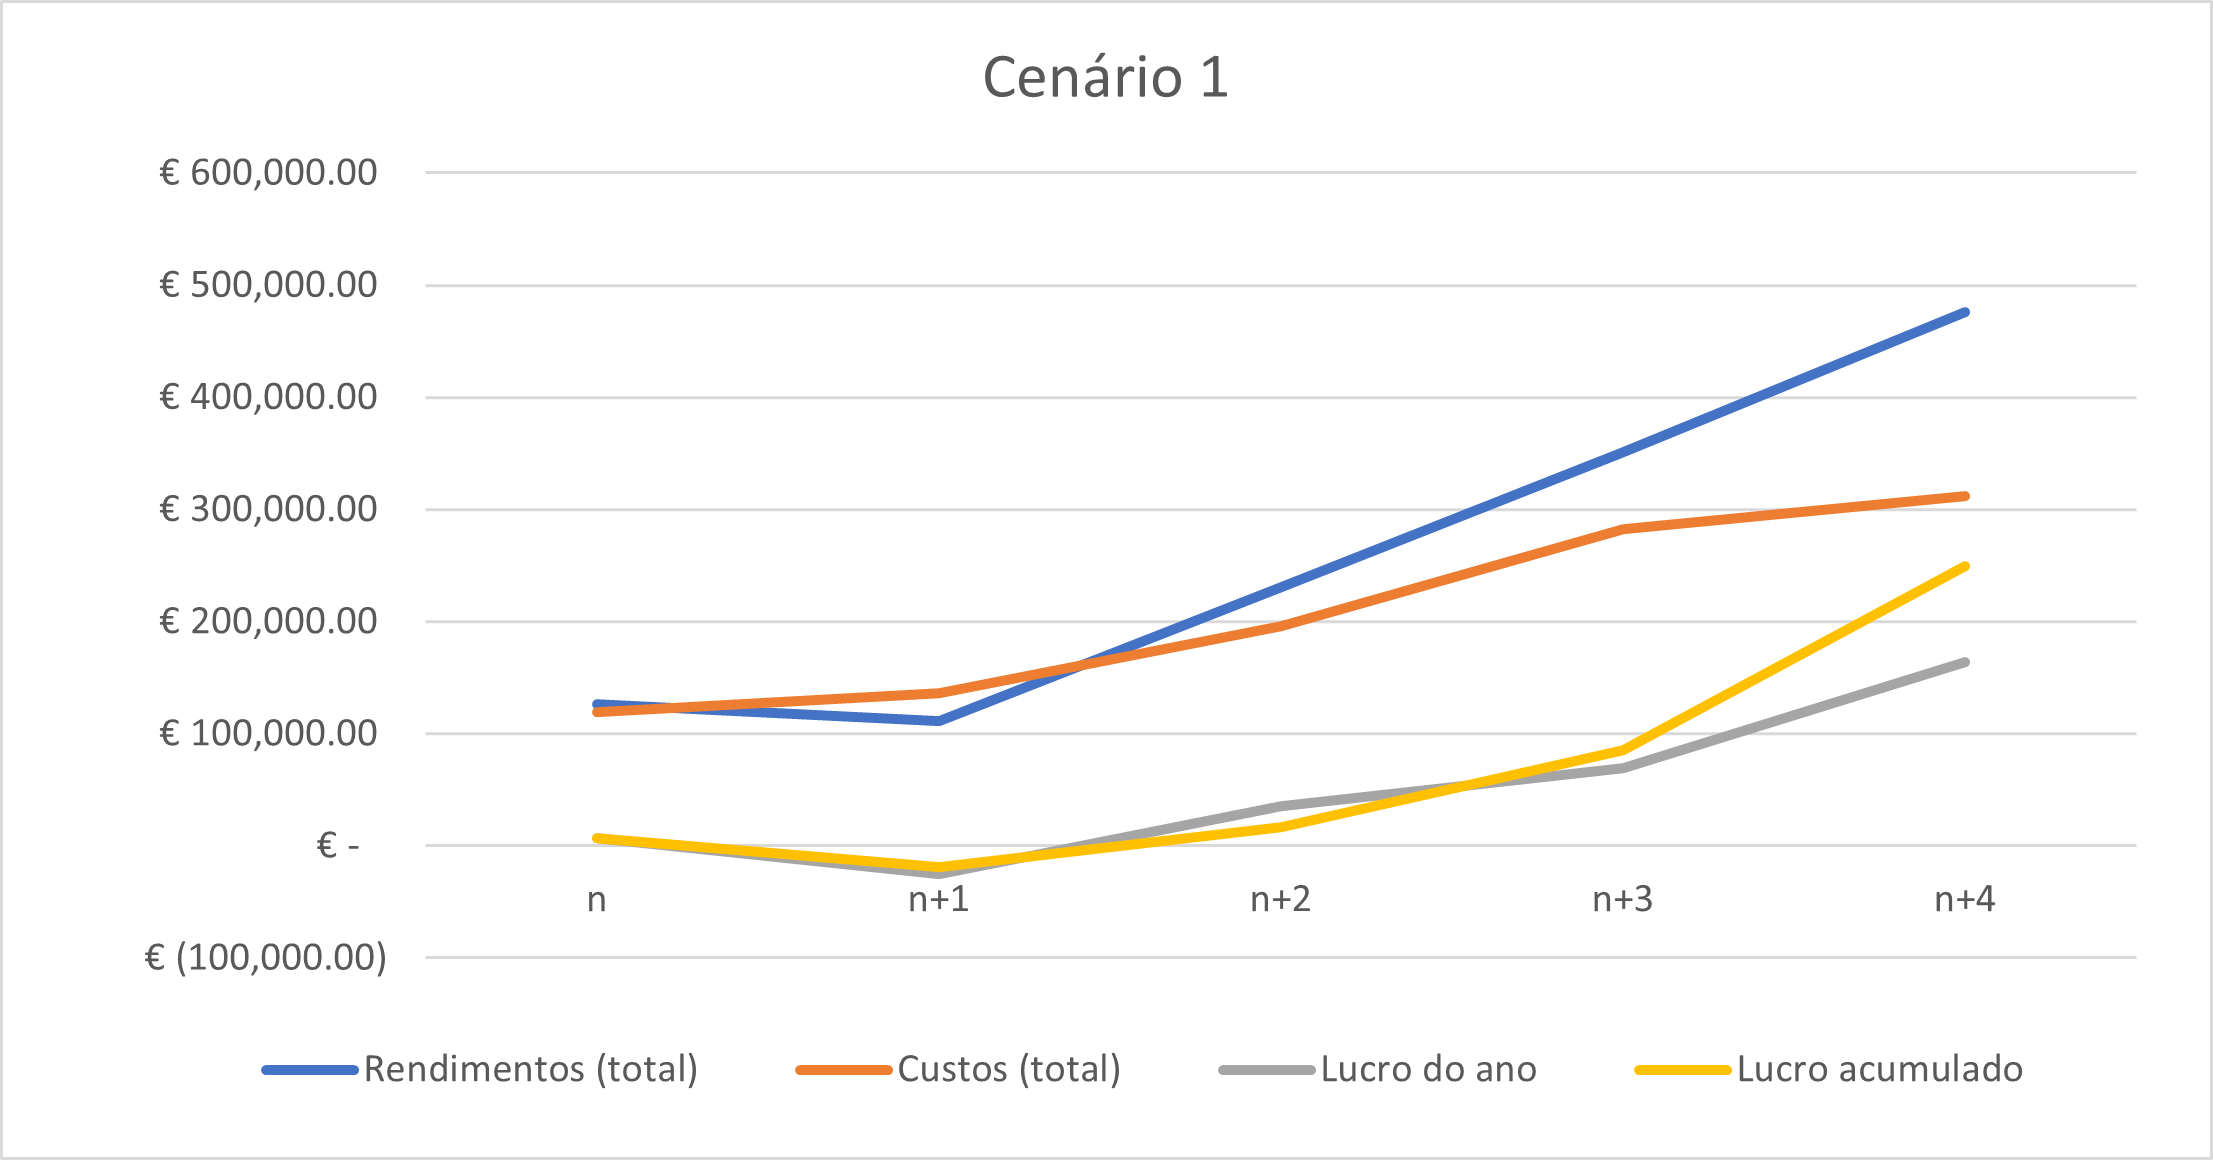
\includegraphics[width = 90mm]{img/graphs/ppin_graph_1.png}
  \caption{Gráfico ilustrativo das previsões a nível financeiro para o cenário descrito como otimista}
\end{figure}

\vspace{-0.5em}

\begin{figure}[ht]
  \centering
  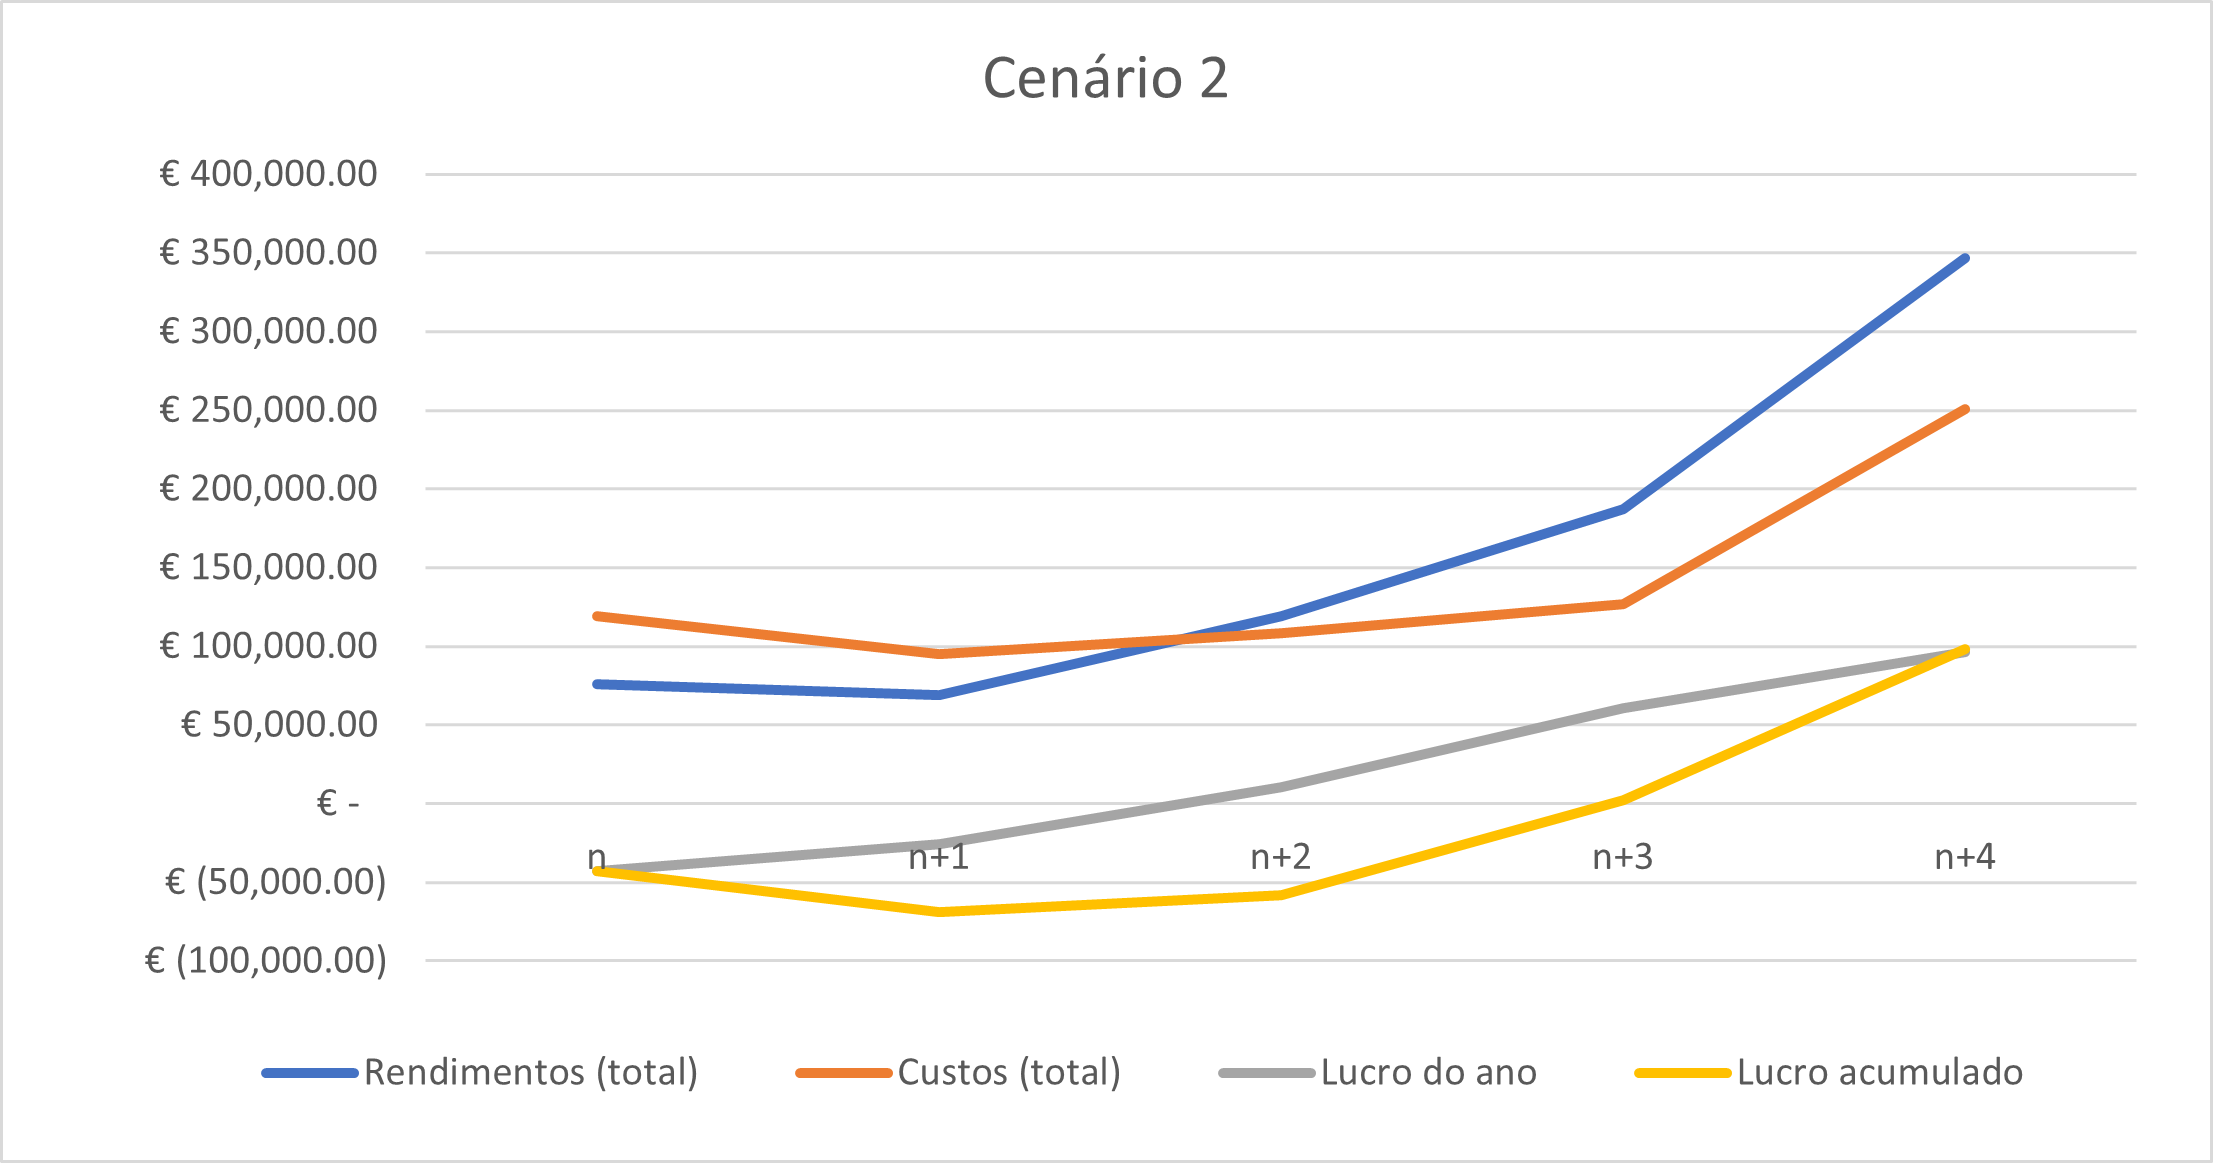
\includegraphics[width = 90mm]{img/graphs/ppin_graph_2.png}
  \caption{Gráfico ilustrativo das previsões a nível financeiro para o cenário descrito como neutro}
\end{figure}

\vspace{-0.5em}

\begin{figure}[ht]
  \centering
  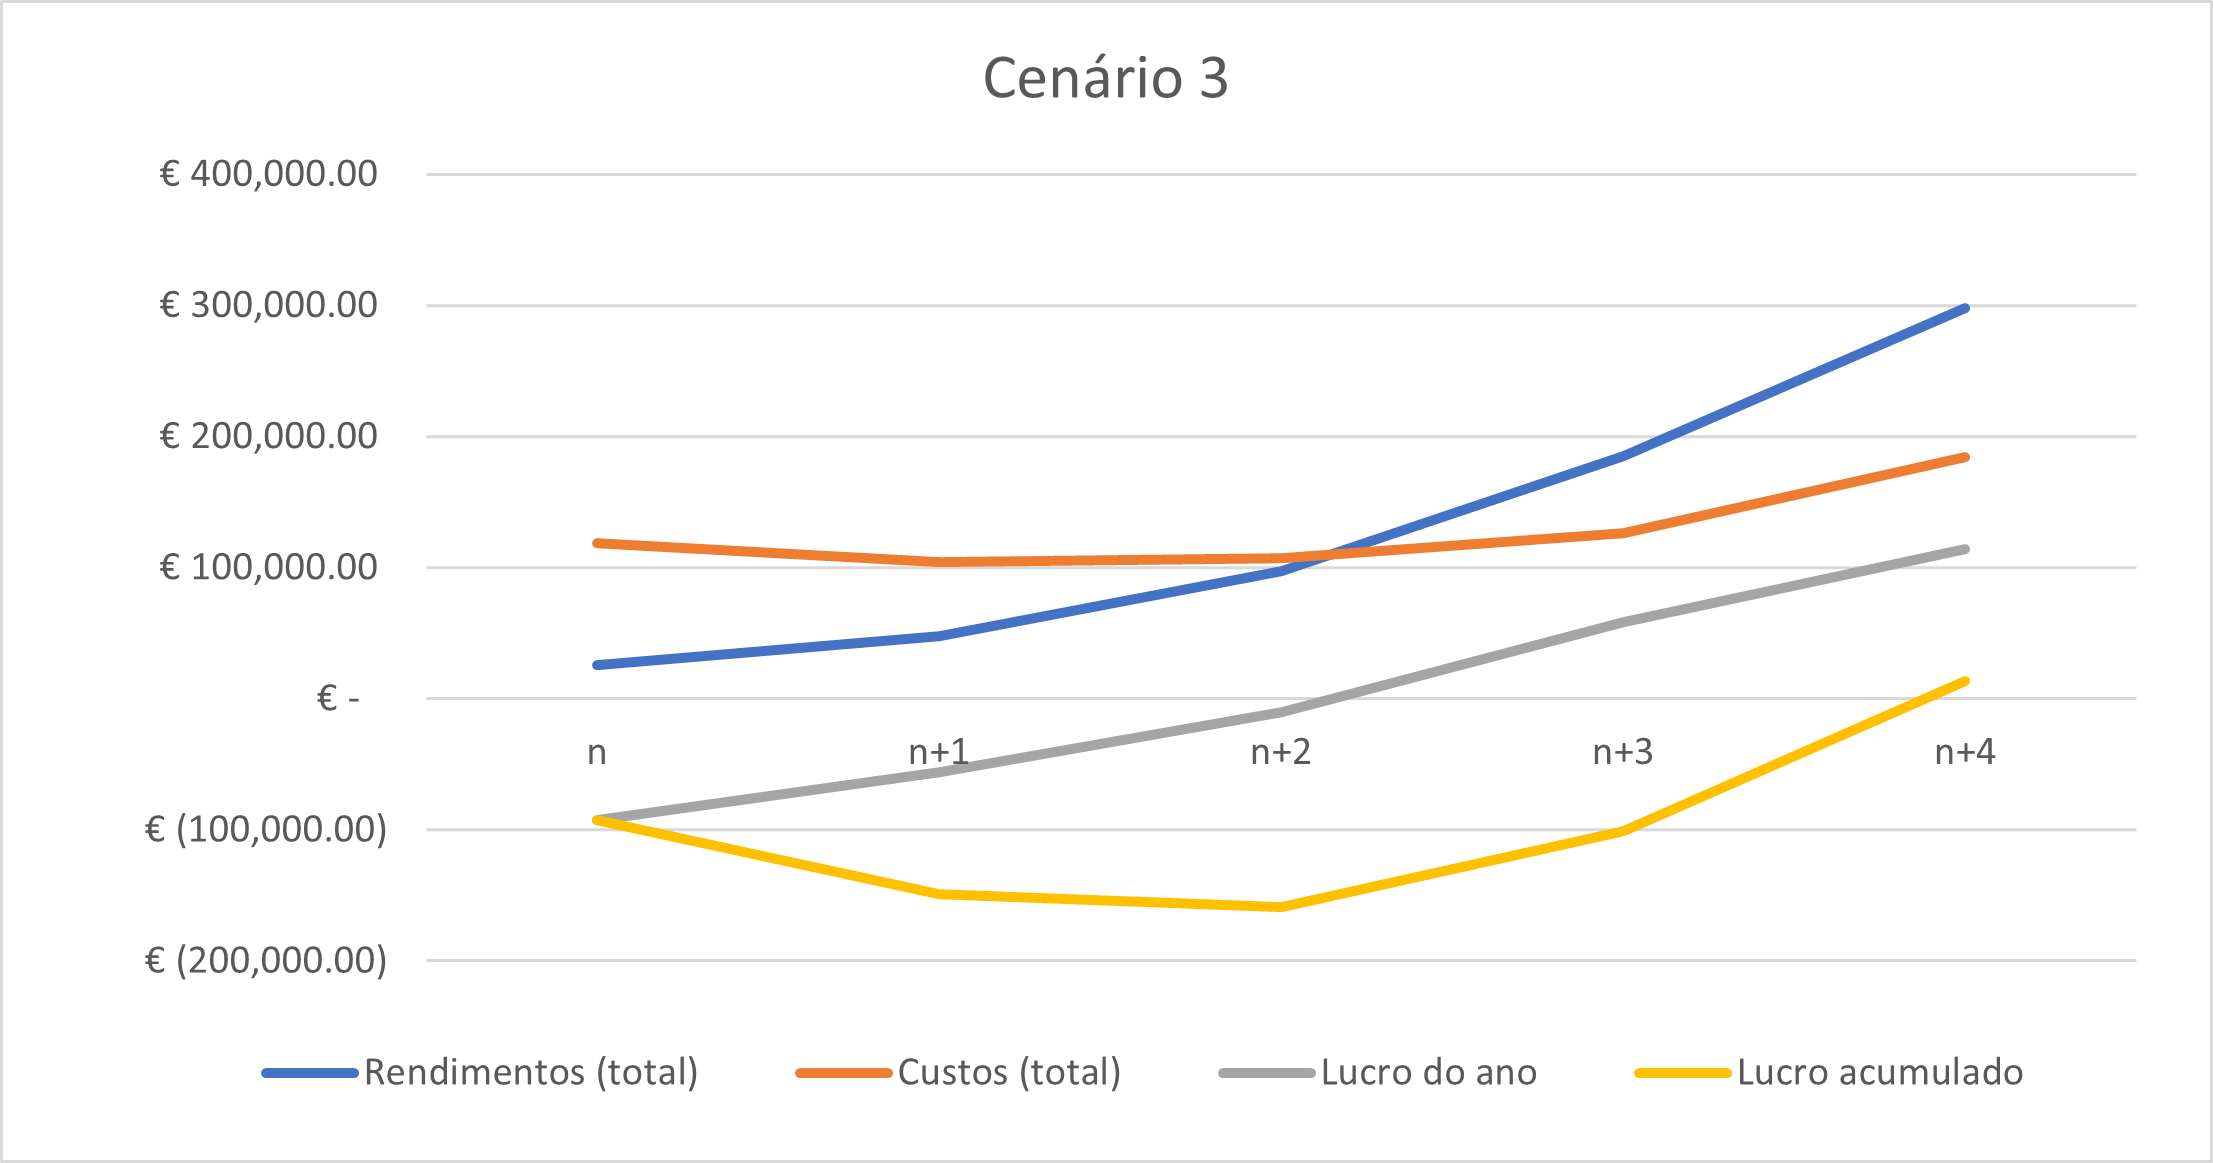
\includegraphics[width = 90mm]{img/graphs/ppin_graph_3.png}
  \caption{Gráfico ilustrativo das previsões a nível financeiro para o cenário descrito como pessimista}
\end{figure}


\chapter{Diário de bordo}

Neste anexo são apresentados as datas e os resumos das reuniões e do trabalho desenvolvido pelos membros do grupo, do momento de sua formação à entrega do trabalho final.

As reuniões realizaram-se de forma remota dada a situação pandémica, durante as aulas da unidade curricular PPIN e também através de chamadas na aplicação Discord, onde foi criado um servidor para comunicação informal entre reuniões, através de mensagens.

\section{Planeamento}

{
\renewcommand{\arraystretch}{1.5}
\begin{tabular}{@{~~} !{\foo} >{\raggedright\arraybackslash}l p{130mm}}
\addlinespace[1.5ex]
\textbf{22/03/2021} & Formação do grupo, após demostração de interesse por parte de todos os membros, no desenvolvimento de um projeto com ênfase no ambiente. \\
\textbf{25/03/2021} & Primeira reunião após a formação do grupo. Foram expostas as opiniões e vontades individuais de cada um frente ao projeto, assim como a primeira discussão sobre ideias de temas a serem escolhidos. Ficou acordado entre os membros de desenvolver uma elaboração das ideias individuais de tema, para na próxima reunião ser realizada uma apresentação interna e decisão do tema. \\
\textbf{29/03/2021} & Foram apresentados possíveis temas, por três integrantes do grupo: Desflorestação, Recolha de Resíduos e Separação de Resíduos com Inteligência Artificial. Após avaliação e votação de todos foi escolhida a Recolha de Resíduos.\\
\textbf{01/04/2021} & Primeira apresentação do tema, em aula.\\
\textbf{05/04/2021} & Reunião em seguimento da apresentação, debateu-se as críticas dos colegas, e possíveis soluções a estas. Foram separadas tarefas relativas a pesquisa de tecnologias semelhantes a proposta do trabalho, já existentes, para serem debatidas na próxima reunião.\\
\textbf{12/04/2021} & Em reunião foram revisadas as pesquisas sobre tecnologias e concorrência existentes. Assim como a discussão sobre legislações vigentes, e diferença de funcionamento do recolhimento de lixo em diferentes concelhos.\\
\textbf{17/04/2021} & Reunião final da fase de planeamento: foi analisado o desempenho desta fase e feito do planeamento da próxima fase. O formato do projeto foi estabelecido e as próximas etapas seriam a pesquisa aprofundada e desenvolvimento dos detalhes do funcionamento do produto por exemplo como seria a aplicação e se seria usada uma etiqueta NFC ou outra tecnologia. \\
\end{tabular}
}

\section{Desenvolvimento - Desafios Tecnológicos}

{
\renewcommand{\arraystretch}{1.5}
\begin{tabular}{@{~~} !{\foo} >{\raggedright\arraybackslash}l p{130mm}}
\addlinespace[1.5ex]
\textbf{21/04/2021} & Reunião inicial da fase, foram debatidas as diferentes possíveis tecnologias a serem usadas como de travas elétricas nos caixotes, etiquetas NFC's vs QR codes, dispositivos para pesagem de lixo. Foram separadas essas tecnologias para serem pesquisadas mais a fundo pelos membros e serem apresentadas na próxima reunião. \\
\textbf{24/04/2021} & Foram apresentadas em reunião os pontos pesquisados, e decididas as tecnologias a serem usadas. Assim como desenvolvido o plano de ação para a próxima fase.
\end{tabular}
}

\section{Desenvolvimento - Análise de Sustentabilidade}

{
\renewcommand{\arraystretch}{1.5}
\begin{tabular}{@{~~} !{\foo} >{\raggedright\arraybackslash}l p{130mm}}
\addlinespace[1.5ex]
\textbf{27/04/2021} & Reunião inicial da fase: foram debatidos os planos de negócio do projeto sua relação com as entidades responsáveis, e o funcionamento distinto relativo ao método de recolha de lixo nos diferentes concelhos. Ficou decidido que seria pesquisado melhor as vantagens e desvantagens das ideias apresentadas e seria decidido na próxima reunião o funcionamento. \\
\textbf{01/05/2021} & Foram apresentados os resultados do trabalho no tempo entre a última reunião. Ficou decidido o modelo final de negócios e da comunicação com as entidades. \\
\textbf{07/05/2021} & Reunião final da etapa de Desenvolvimento: foi feita uma avaliação geral do projeto até então. Uma formalização das ideias no primeiro modelo deste relatório e uma preparação para a etapa de realização. 
\end{tabular}
}

\section{Realização}

{
\renewcommand{\arraystretch}{1.5}
\begin{tabular}{@{~~} !{\foo} >{\raggedright\arraybackslash}l p{130mm}}
\addlinespace[1.5ex]
\textbf{10/05/2021} & Foram dividias as tarefas relativas a realização do relatório final, da apresentação e dos trabalhos envolvidos nestes.\\
\textbf{13/05/2021} & Durante a reunião durante a aula foi discutida a ideia de enviar um inquérito através do e-mail dinâmico. Todos os membros do grupo concordaram que seria benéfico para a realização do projeto.\\
\textbf{15/05/2021} & Reunião para a elaboração do inquérito. Ficou decidido que seriam dez questões, relativas aos hábitos dos estudantes quanto a reciclagem e sua disposição para aderir ao projeto.\\
\textbf{16/05/2021} & Envio do inquérito através do e-mail dinâmico\\
\textbf{19/05/2021} & Reunião pré apresentação final: foi revisto o resultado do inquérito, a trabalho desenvolvido e foi dividido o que cada membro iria falar na apresentação.\\
\textbf{20/05/2021} & Apresentação final do trabalho \\
\end{tabular}
}

\chapter{Mockups do protótipo}
\label{ch:anexo-mockups}

Apresentam-se de seguida os mockups do protótipo da aplicação móvel e da web app.

\subsubsection{Aplicação móvel}

\begin{figure}[h!]
    \centering
    
    \begin{subfigure}[t]{0.33\textwidth}
        \centering
        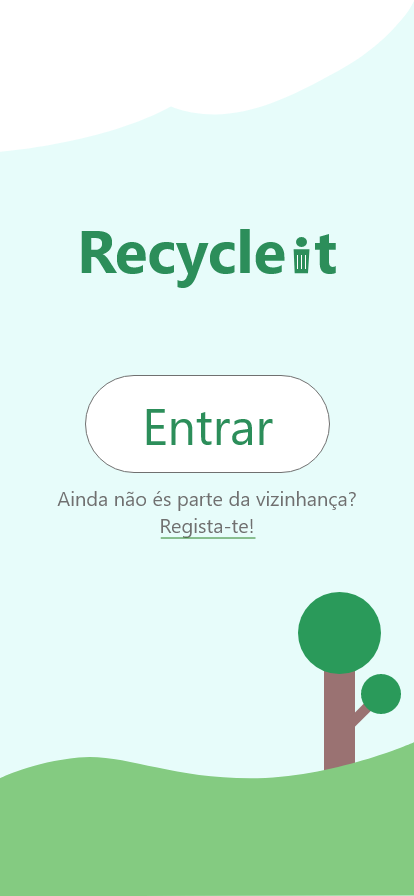
\includegraphics[width=52mm]{img/mockups/tlmv-1.png}
        \caption{Ecrã de entrada}
    \end{subfigure}%
    \begin{subfigure}[t]{0.33\textwidth}
        \centering
        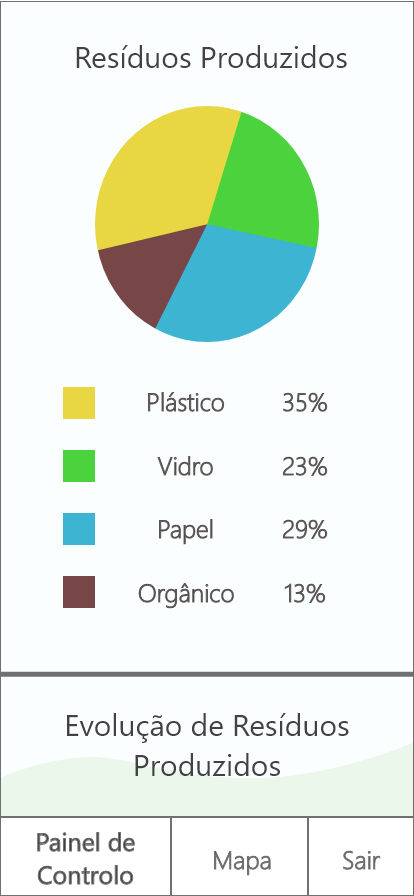
\includegraphics[width=52mm]{img/mockups/tlmv-2.png}
        \caption{Consulta do lixo produzido}
    \end{subfigure}%
    \begin{subfigure}[t]{0.33\textwidth}
        \centering
        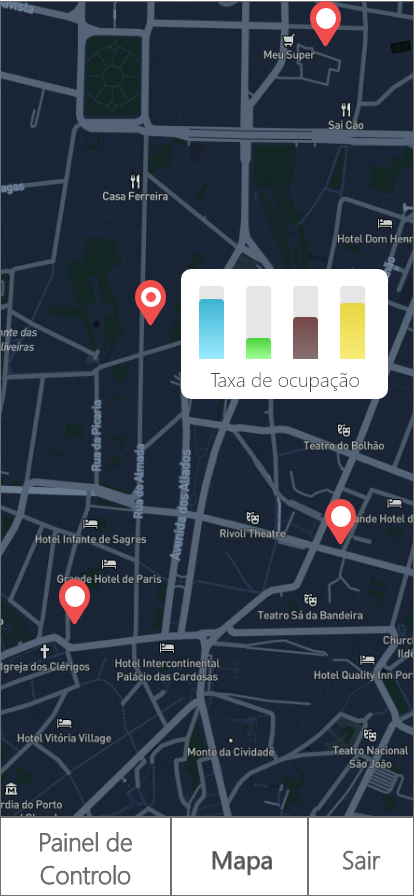
\includegraphics[width=52mm]{img/mockups/tlmv-3.png}
        \caption{Consulta dos ecopontos}
    \end{subfigure}
    
    \caption{Mockups do protótipo da aplicação móvel}
\end{figure}

\newpage

\subsubsection{Web app}

\begin{figure}[h!]
    \centering
    
    \begin{subfigure}[t]{0.99\textwidth}
        \centering
        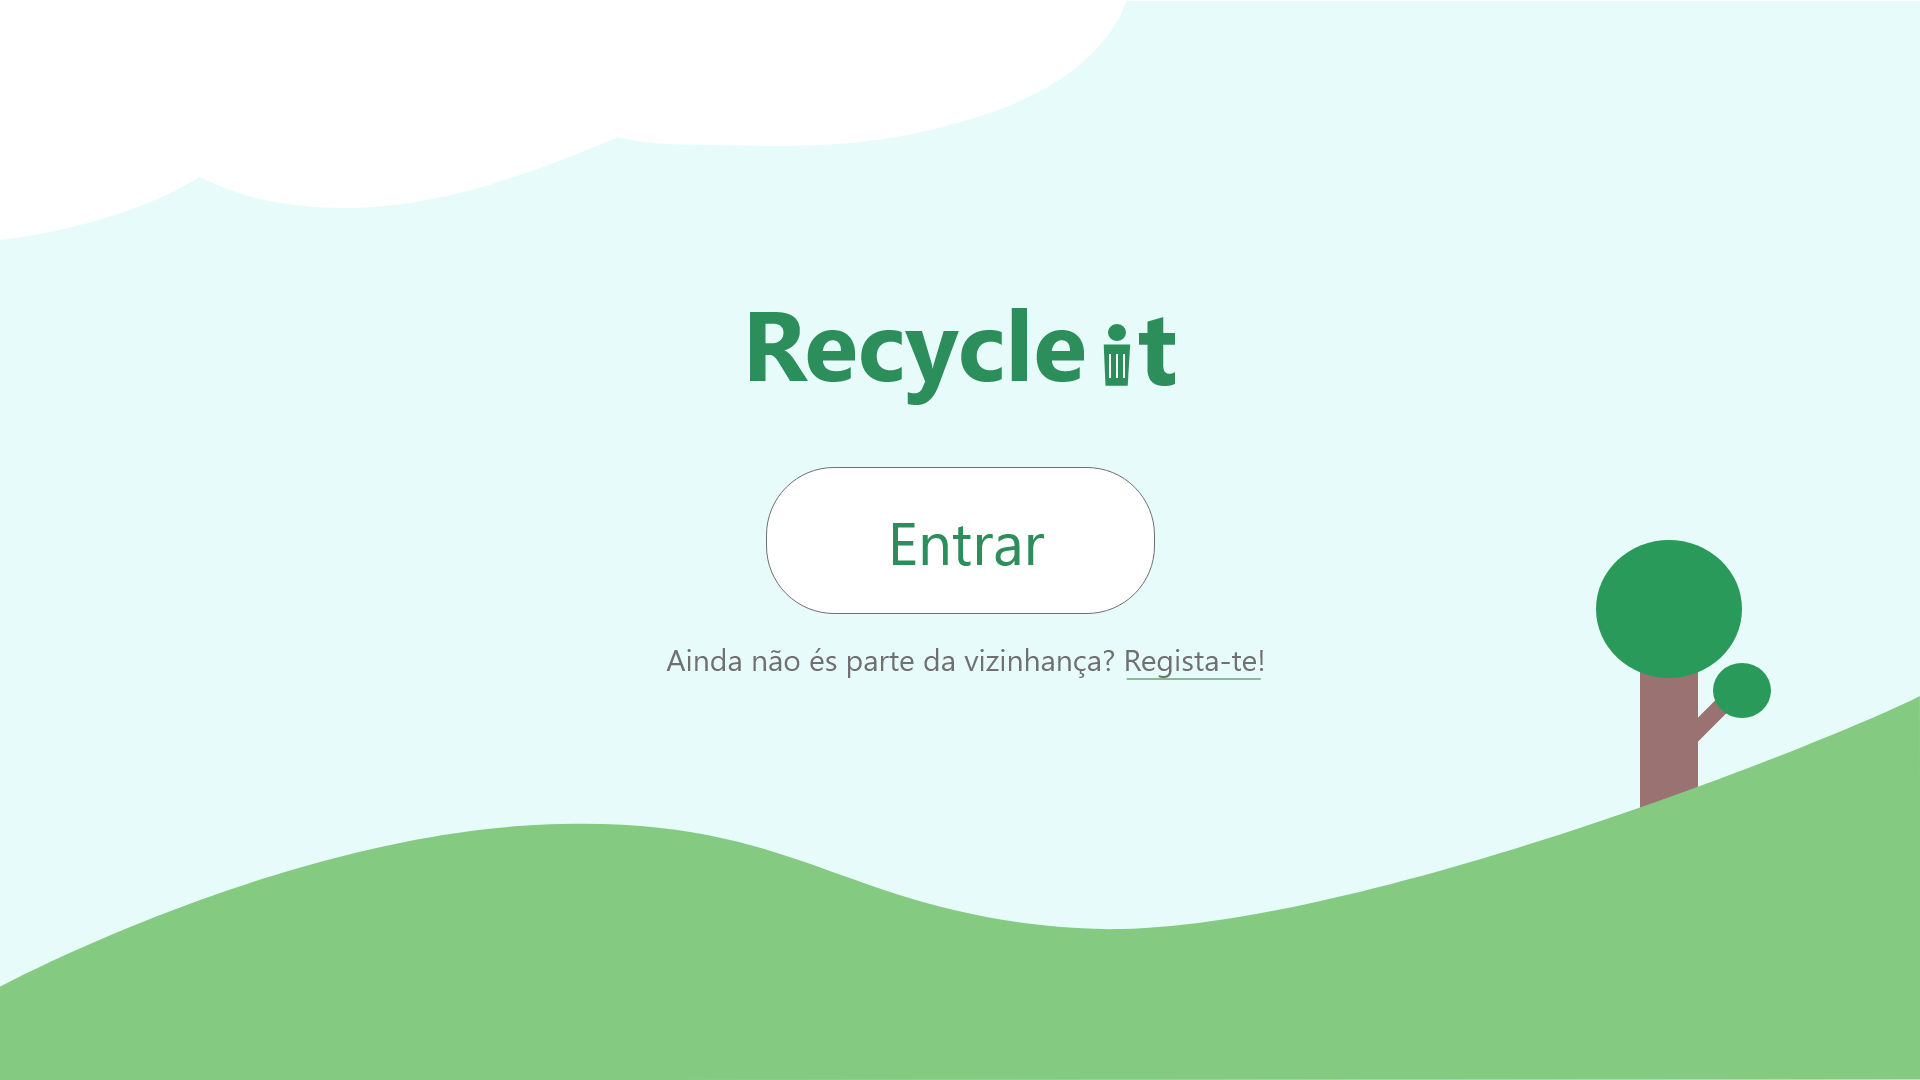
\includegraphics[width=120mm]{img/mockups/web-1.png}
        \caption{Ecrã de entrada}
    \end{subfigure}
    \begin{subfigure}[t]{0.99\textwidth}
        \centering
        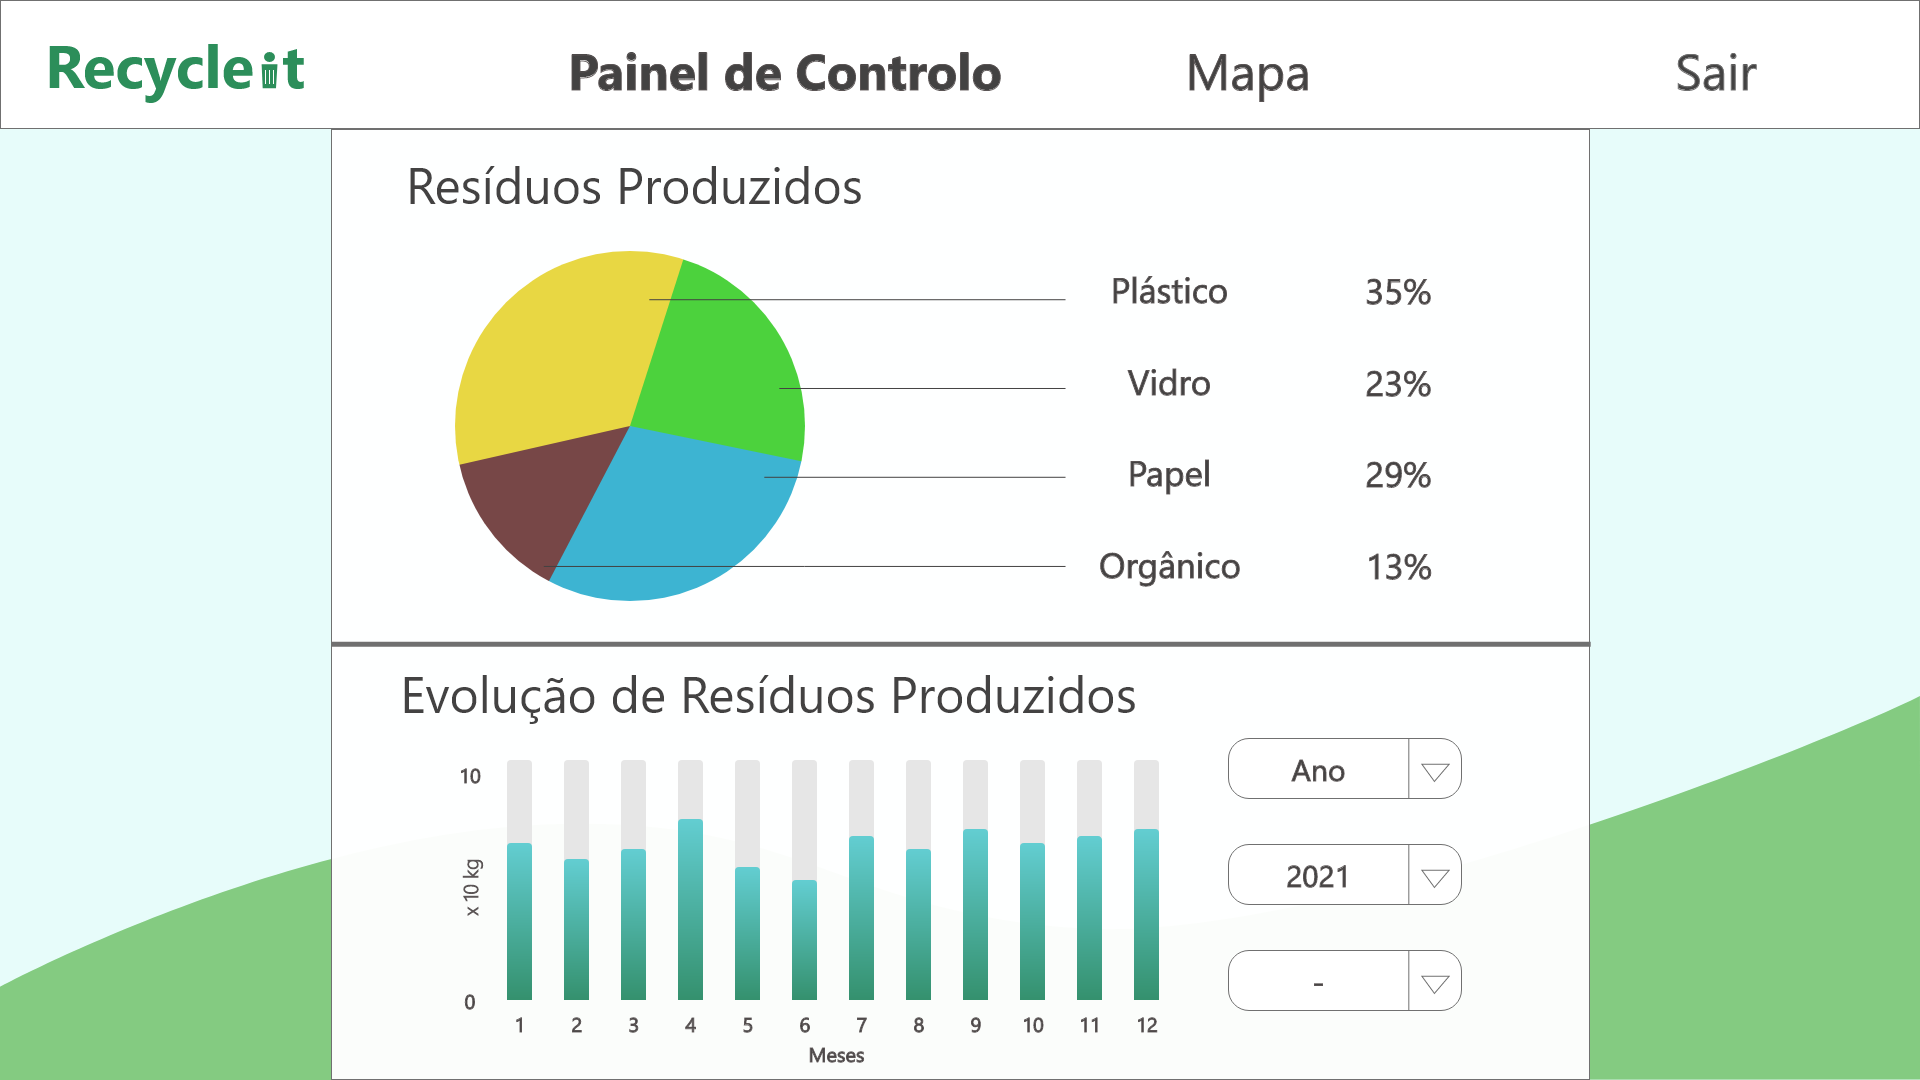
\includegraphics[width=120mm]{img/mockups/web-2.png}
        \caption{Consulta do lixo produzido}
    \end{subfigure}
    \begin{subfigure}[t]{0.99\textwidth}
        \centering
        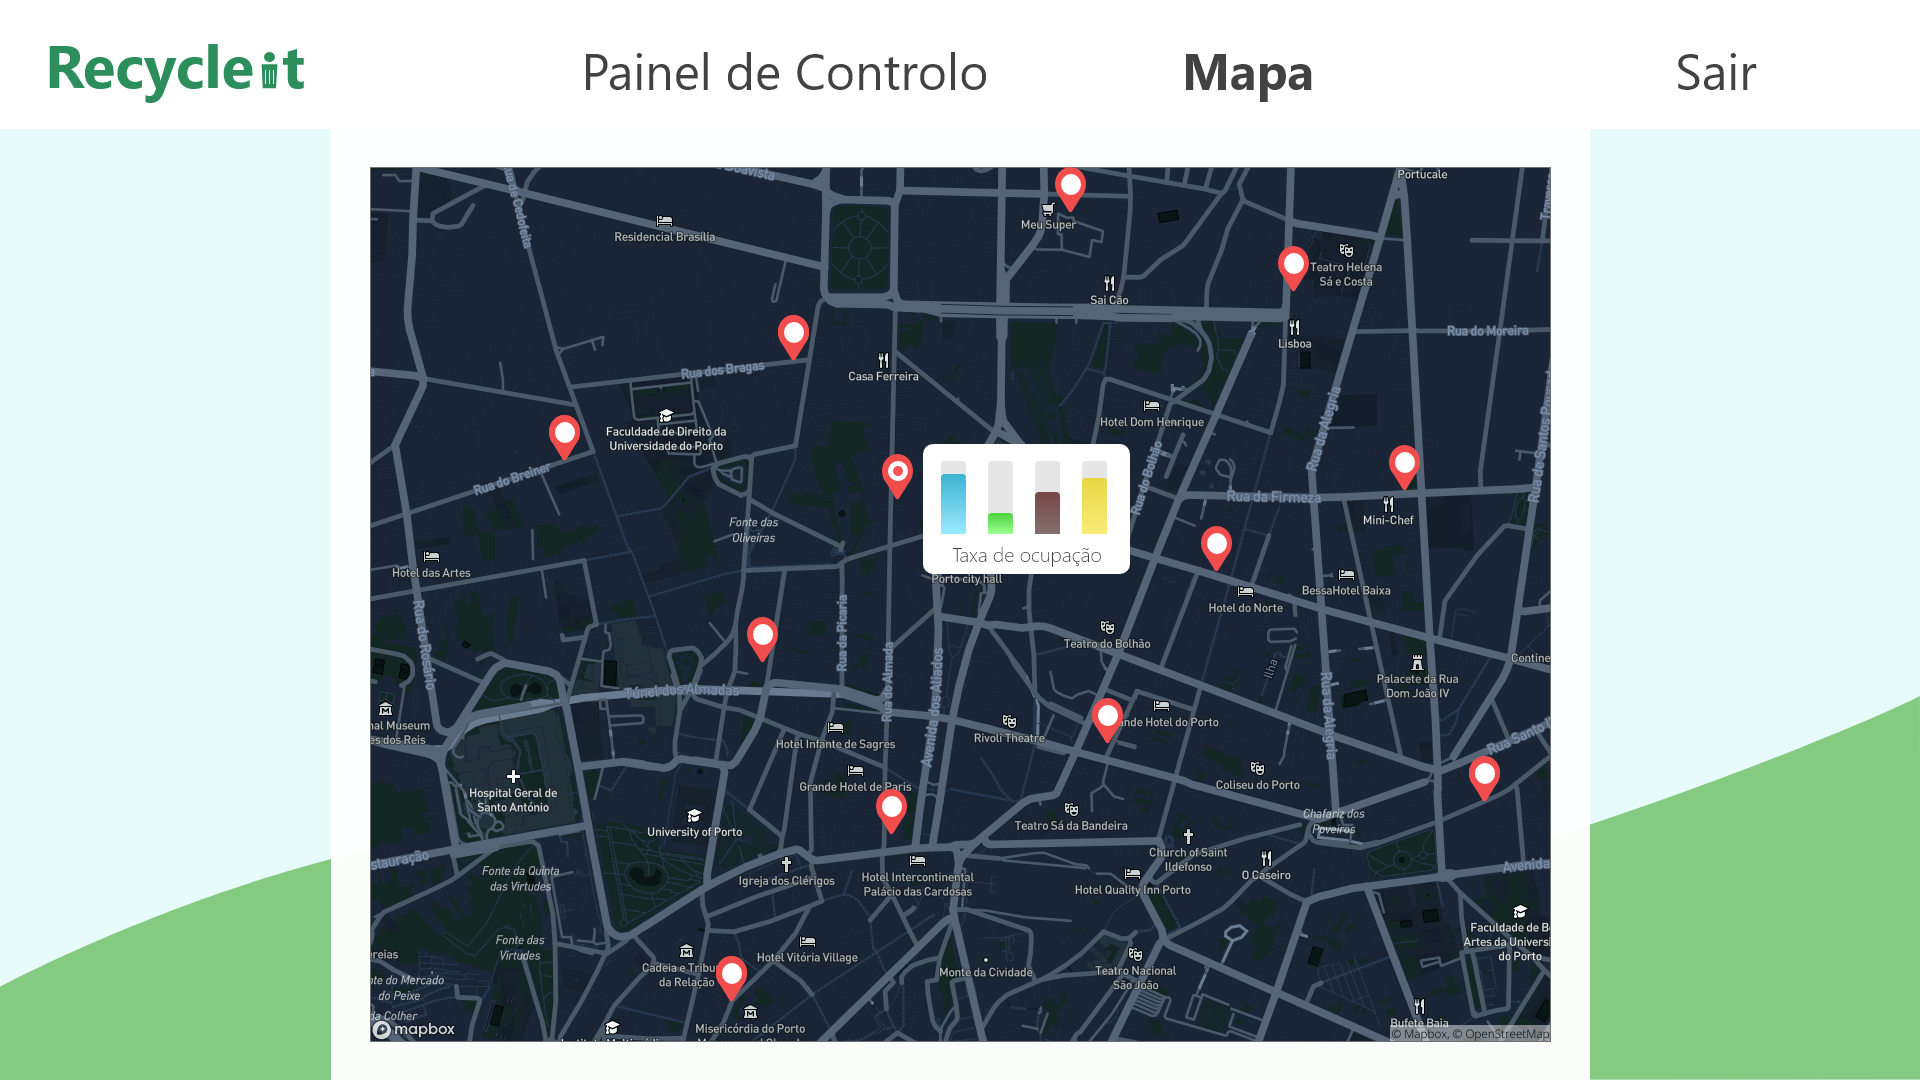
\includegraphics[width=120mm]{img/mockups/web-3.png}
        \caption{Consulta dos ecopontos}
    \end{subfigure}
    
    \caption{Mockups do protótipo da web app}
\end{figure}

\chapter{Media}

Segue-se o \textit{media} deste projeto, que consiste nas várias versões do logótipo. A cor verde é trocada por branco (e a cor branca é trocada por transparência, como nos traços do caixote de lixo no "i") quando é necessário colocar o logótipo sobre um fundo não-branco.

\subsubsection{Logótipo completo}

\begin{center}
    
\includegraphics[scale=2.0]{img/recycle-it-full.png}
\end{center}

\subsubsection{Logótipo pequeno}

\begin{center}
    
\includegraphics[scale=2.0]{img/recycle-it.png}
\end{center}

\end{appendices}

\end{document}
